% $Id: CONTENT.tex 10532 2010-03-16 15:57:20Z alexandra $
% Local Variables:
% ispell-check-comments: nil
% Local IspellDict: american
% End:
% --------------------------------------------------------
% User documentation
% copyright by BREDEX GmbH 2005
% --------------------------------------------------------
% this command can be inserted multiple times
%\gdhelpid{}
% 
%\begin{gddescription}
%\end{gddescription}
%
%\begin{gdlist}
% use the \item command for single steps
%\end{gdlist}
% change <PATH> to the same directory, file is located in
% change <FILE> to the same filename you are editing
%\bxinput{<PATH>/Links/<FILE>}
%
% other usefull commands are
%   \bxtipp{}        to create a hint
%   \bxwarn{}        to describe a warning
\index{Observation Mode}

\subsection{Tips and tricks for using the observation mode}
\label{TasksObsModeTips}
\index{Observation Mode!Tips}

We have designed the \jb{} observation mode to help you get started with your tests and to help you understand what sort of user actions correspond to \jb{} actions. 

\jb{} is first and foremost a keyword-driven tool, and the library of \gdcases{} installed with \jb{} means that you have various benefits over simple recording:

\begin{itemize}
\item You can create tests without needing the \gdaut{} - you don't have to wait for each version of the \gdaut{} to begin test specification. 
\item Your tests aren't so dependent on the actual implementation of the \gdaut{}, so they can be a lot more general in terms of data, component implementations etc. and therefore a lot more robust and maintainable. 
\item Using keywords encourages you to think about your test structure a lot more, which also helps maintenance later. 

\end{itemize}


Nevertheless, we understand that you may want to observe some \gdcases{}. Here are some tips that might help you:
\begin{itemize}
\item Think about your test structure at the beginning: what modules will you want to reuse? Start by observing small \gdcases{}, e.g. a \gdcase{} to login, a \gdcase{} to open a dialog etc. 
\item Check while you are observing that the actions you carry out are observed in the way you meant. 
\item Supplement your observed \gdcases{} with other \gdcases{} from the library of \gdcases{} in \jb{}. 
\item Refactor as you go! If you have recorded a \gdcase{} with specific data, but you will want to use it for any type of data, then add a reference for the data. 
\end{itemize}


\subsection{Starting observing}
% BREDEX LaTeX Template
%  \documentclass is either ``bxreport'' or ``bxarticle''
%                 option is bxpaper
%% \documentclass{bxarticle}
%% % ----------------------------------------------------------------------
%% \begin{document}
%% \title{}
%% \author{}
%% % \author*{Hauptautor}{Liste der Nebenautoren}
%% \maketitle
%% % ----------------------------------------------------------------------
%% \bxversion{0.1}
%% %\bxdocinfo{STATUS}{freigegeben durch}{freigegeben am}{Verteilerliste}
%% \bxdocinfo{DRAFT}{}{}{}
%% % ----------------------------------------------------------------------

%% \end{document}
\index{Observation Mode!Start}
\index{Start!Observation Mode}
\label{startobs}
To be able to observe \gdsteps{}, you must:
\begin{itemize}
\item define an \gdaut{} \bxpref{Defineaut}
\bxtipp{Only Java \gdauts{} can use the observation mode. }
\item configure an \gdaut{} \bxpref{configuringaut} if you want to start it via \app{}. 
\item set the working language to the language you want to observe in.
\item start the \gdaut{} you want to observe from \bxpref{startaut} (either via a configuration \bxpref{configuringaut} or using the \bxname{autrun} command \bxpref{autrun}). 
\end{itemize}

Once you have completed these steps, you can select the \bxcaption{observe \gdcase{}} button 
\gdmarpar{../../../share/PS/cam}{start observation}
on the main toolbar.
\begin{enumerate}
 \item When asked, enter a name for the observed \gdcase{}.
 \item The status bar will show that you are in the observation mode. 
 \item A \gdtestcaseeditor{} for the observed \gdcase{} will appear. 
 \item Switch to the \gdaut and activate it by clicking once in the title bar.
 \item You can now observe \gdsteps{}.
\bxtipp{If you have a \gdcase{} open in the \gdtestcaseeditor{}, the \gdsteps{} will be observed into this open \gdcase{}. }
\end{enumerate}


 


 


\subsection{Observing tests in Java \gdauts{}}
\index{Observing!Test Steps}
\index{Test Step!Observe}
\label{TasksObserveJava}

\bxtipp{If you have not already done so, we recommend reading the tips section for the observation mode before beginning observing \bxpref{TasksObsModeTips}. }
\begin{enumerate}
\item  In Java \gdauts{} (Swing and SWT/RCP) the observation mode will automatically record your actions in the user interface. Each action is created as a \gdstep{} in the \gdtestcaseeditor{} for this observed \gdcase{}. 

\bxtipp{See the section later on performing check actions in the observation mode \bxpref{TasksObsCheckJava}.}

\item You can also see which actions have been recorded in the console (\bxfigref{obsconsole}).

\begin{figure}[h]
\begin{center}
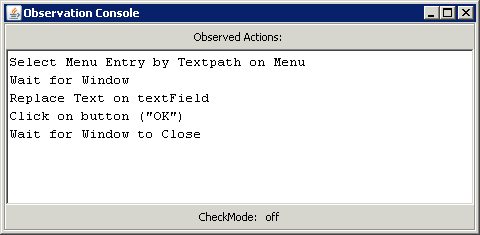
\includegraphics{Tasks/Recording/PS/obsconsole}
\caption{The observation console}
\label{obsconsole}
\end{center}
\end{figure}


\bxtipp{If you are creating tests for SWT and RCP \gdauts{}, check that you have set the keyboard layout correctly in the \gdproject{} properties \bxpref{AdvancedAUTConfig} and that you have defined the right toolkit for the \gdproject{} \bxpref{ProjPropertiesChangingToolkit}.}
 

\item Component names for your components are automatically generated and assigned to the technical names from the \gdaut{} when you observe \gdsteps{}. If \app{} notices that you have already created and mapped a component name for a technical component, it will use this name instead of creating a new one. 
\item Once you have recorded the actions you need, stop the observation mode by clicking on the \bxcaption{stop observing \gdcase{}} button 
\gdmarpar{../../../share/PS/stopcam}{stop observation}
on the main toolbar.
\item Save the \gdcase{} editor containing the \gdsteps{} you have just observed. 
\item Check the \gdsteps{} and their parameter values which have been recorded. 
You will notice that any text that contains non-alphanumeric characters is enclosed in single quotes. Single quotes are used by \app{} to cancel any meaning of the characters within the quotes. 
\bxtipp{Run the test that you have just recorded to see if it works as you intended. If not, you may need to make some changes to the parameter values, or you may have to supplement the \gdcase{} with \gdcases{} from the library \bxpref{UseLibrary}. }
\end{enumerate}

\subsubsection{Actions that cannot be recorded}
A few actions cannot be recorded in the current version. These include:
\begin{itemize}
\item Key combinations that are used as shortcuts in SWT applications.
\item Click counts on trees. The select actions are correctly recorded, but the click count is set to 0 and must be manually adjusted. 
\item Components that contain texts that are too long (more than 3999 characters). 
\item Actions on native dialogs e.g. file choosers. 
\end{itemize}

\subsubsection{Performing checks in the Java observation mode}
\label{TasksObsCheckJava}

You can perform checks in the observation mode by taking the following steps:
\begin{enumerate}
\item Start the check mode by pressing \bxkey{Ctrl+Shift+F11}. This key combination can be changed in the preferences \bxpref{TasksPrefsObsModeJava}. 
\item In the observation console, the check mode will be marked as \bxname{on}. 
\item In the \gdaut{}, components will be highlighted with a red border (\bxfigref{redborders}).

\begin{figure}[h]
\begin{center}
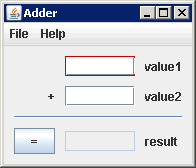
\includegraphics{Tasks/Recording/PS/redborders}
\caption{Red borders in the check  mode}
\label{redborders}
\end{center}
\end{figure}
 
\bxtipp{While the check mode is active, no other actions will be recorded.}
\item Hover over the component you want to execute a check on and press \bxkey{Ctrl+Shift+F12}. This key combination can be changed in the preferences \bxpref{TasksPrefsObsModeJava}. 
\item A dialog will appear showing the type of component you are performing the check on. 
\item From the dialog, select the check action you want to perform and enter any parameters the check action needs. Many check actions have predefined parameters based on the state of the \gdaut{}. 
\item When you have specified your check action, choose whether you want to close the dialog and continue in the check mode (\bxname{check on}) or whether you want to stop the check mode when the dialog closes (\bxname{stop checking}). 
\bxtipp{You can manually stop the check mode using the same key combination as you used to start the check mode (\bxkey{Ctrl+Shift+F11} by default).}
\item The check action you specify will be added to the \gdtestcaseeditor{}. 
\end{enumerate}




  




%% \subsection{Observing tests in HTML \gdauts{}}
%% \label{TasksObserveWeb}
The observation mode for HTML \gdauts{} involves hovering over the component you want to record an action on and pressing a key combination to execute an action on this component:
\begin{itemize}
\item Press  \bxkey{Ctrl+Shift+A} to map that component. 
\item Press \bxkey{Ctrl+Shift+S} to map the application component. 
\end{itemize}

Supported components are marked with red borders (\bxfigref{redborders}). 

\begin{figure}[h]
\begin{center}
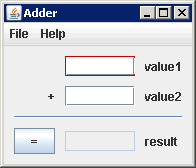
\includegraphics{Tasks/Recording/PS/redborders}
\caption{Red borders in the observation mode}
\label{redborders}
\end{center}
\end{figure}

In the dialog which appears, choose the action you want to execute on this component.

Once you have done this, you can:
\begin{enumerate}
\item Enter the parameters for the action, as prompted by the dialog box.
\bxtipp{You can only enter concrete parameter values in this dialog.}
\item Click \bxcaption{OK} in the dialog.
\item The action you just specified will be carried out.
\item In the \gdtestcaseeditor{} for the \gdcase{} you are observing, the \gdstep{} you just observed will appear. 
\item In the \gdpropview{}, you will see that the \bxname{component} name field contains a name generated by \gd{}. This component name is assigned to the technical name for the component in the \gdomeditor{}. 
\bxtipp{If you change the component name, remember that you will need to reassign your new name to the technical name in the \gdomeditor{}. }
\end{enumerate}

Once you have finished observing your \gdcase{}, stop the observation mode by  
selecting the \bxcaption{stop observing} button on the toolbar. 
 \gdmarpar{../../../share/PS/stopcam}{ stop observation}
\bxtipp{When you are observing, remember that your tests will be more flexible and maintainable if you make the \gdcases{} small, reusable units. }

Save the changes in the editor. 

%checks in the observation mode









%\input{Tasks/Recording/observe}
